\chapter{Introducción específica}

\label{Chapter2}

En este capítulo se detallan las tecnologías que forman parte del trabajo.
Son productos de terceros que integran las herramientas entregadas al cliente.

\section{Arquitectura del dispositivo bajo prueba}
\label{sec:dut}

El trabajo fue realizado para un tipo de microcontrolador específico.
Su diseño forma parte de la familia \emph{Cortex M} de la empresa \emph{ARM}.
En la figura \ref{fig:cortexm} se puede observar un diagrama en bloques de la arquitectura.

Al fabricante del dispositivo bajo prueba se le impone respetar el mapa de memoria y registros del núcleo.
Esto permitió construir un inyector de \emph{soft-errors} genérico.
Finalmente, la herramienta entregada funciona para cualquier integrado de la familia \emph{Cortex M}.

\begin{figure}[htbp]
	\centering
	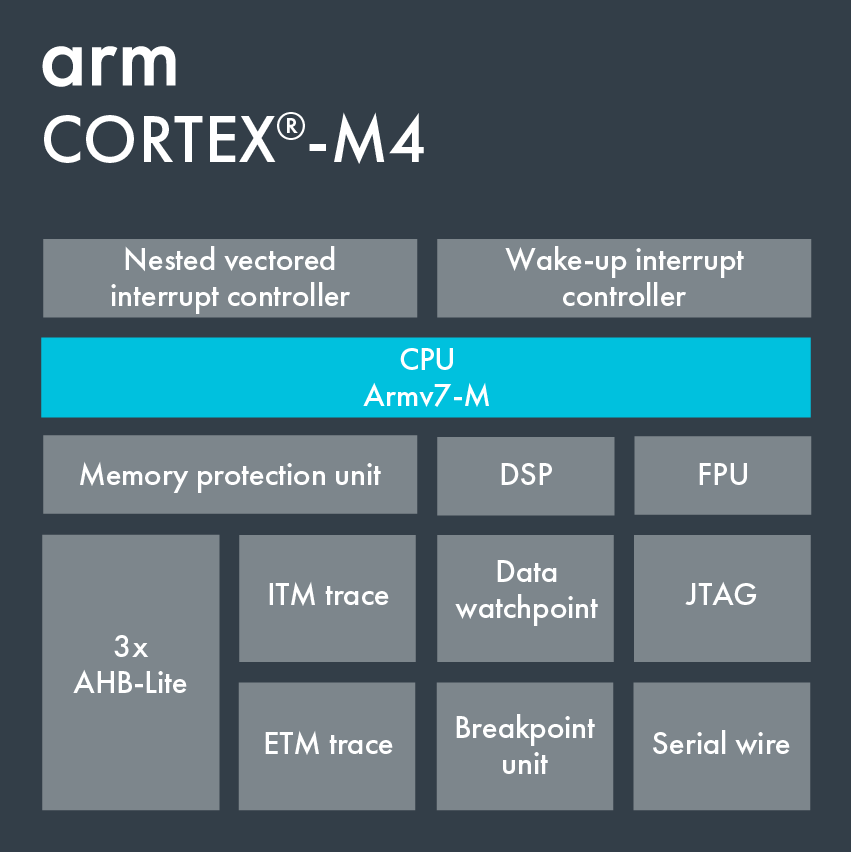
\includegraphics[width=.7\textwidth]{./Figures/Cortex-M4.png}
    \caption{Diagrama de la arquitectura \emph{Cortex M4}\protect\footnotemark.}
	\label{fig:cortexm}
\end{figure}

\footnotetext{Imagen tomada de la página oficial de \emph{ARM Developers}. \citep{WEBSITE:cortexm}}
\newpage

La arquitectura tiene un módulo que permite programar y depurar el integrado.
Este módulo se denomina \emph{CoreSight} y es propio de los dispositivos \emph{ARM}.
En la figura \ref{fig:coresight} se muestra un diagrama en bloques del módulo.
Sus partes principales son:

\begin{itemize}
    \item \emph{Cross Triggering}: permite conectar y encaminar las señales que utilizan las sondas de depuración.  
    \item \emph{Debug Access Port}: es el puerto físico para conectar la sonda de depuración. Es una implementación de la interfaz de depuración \emph{ARM}.
    \item \emph{Embedded Trace Macrocells}: permite extraer información y controlar el núcleo del dispositivo.
    \item \emph{Instrumentation Trace Units}: permite que una sonda de depuración se conecte con las \emph{Embedded Trace Macrocells}.
    \item \emph{ROM Tables}: sirven para que la sonda de depuración identifique al integrado.
    \item \emph{Self Hosted Debug}: son instrucciones específicas de depuración controladas por un procesador secundario.
    \item \emph{Trace Interconnect}: provee puentes para compartir señales de reloj, alimentación y otras señales comunes.
\end{itemize}

\begin{figure}[htbp]
	\centering
	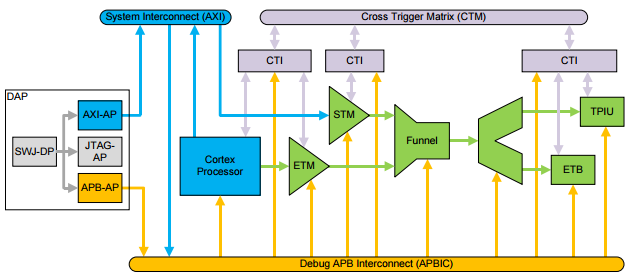
\includegraphics[width=\textwidth]{./Figures/coresight.png}
    \caption{Diagrama del módulo \emph{CoreSight}\protect\footnotemark.}
	\label{fig:coresight}
\end{figure}
\footnotetext{Imagen tomada del artículo \emph{How to debug: CoreSight basis}. \citep{WEBSITE:coresight}}

\section{Servidores y sondas de depuración}
\label{sec:depuracion}

Una sesión de depuración sirve para observar y modificar el estado de ejecución de un programa.
Esto se logra al leer y modificar los valores en registros del procesador y periféricos.
Además, se necesita de un sistema de disparos por eventos y supervisión de recursos.
Finalmente, la sesión debe detener la ejecución del núcleo de ser necesario.
En la figura \ref{fig:debug} se puede observar un esquema simplificado de una sesión de depuración.

\begin{figure}[htbp]
	\centering
	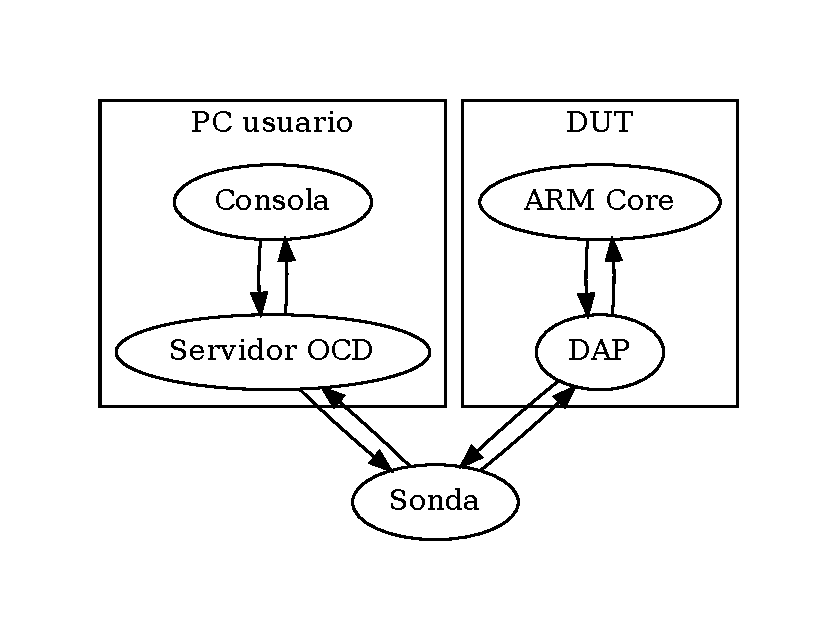
\includegraphics[width=.8\textwidth]{./Figures/debug.pdf}
    \caption{Conexión de una sesión de depuración.}
	\label{fig:debug}
\end{figure}

\newpage

Las sondas de depuración tienen el objetivo de conectar el \emph{Debug Access Port} con el puerto del ordenador del usuario.
Adaptan los niveles de tensión y los protocolos involucrados.
Luego, permiten realizar una sesión de depuración, programar el dispositivo o verificar el estado de los dispositivos en la placa.
En la figura \ref{fig:sonda} se puede ver la sonda provista por el cliente.

\begin{figure}[htbp]
	\centering
	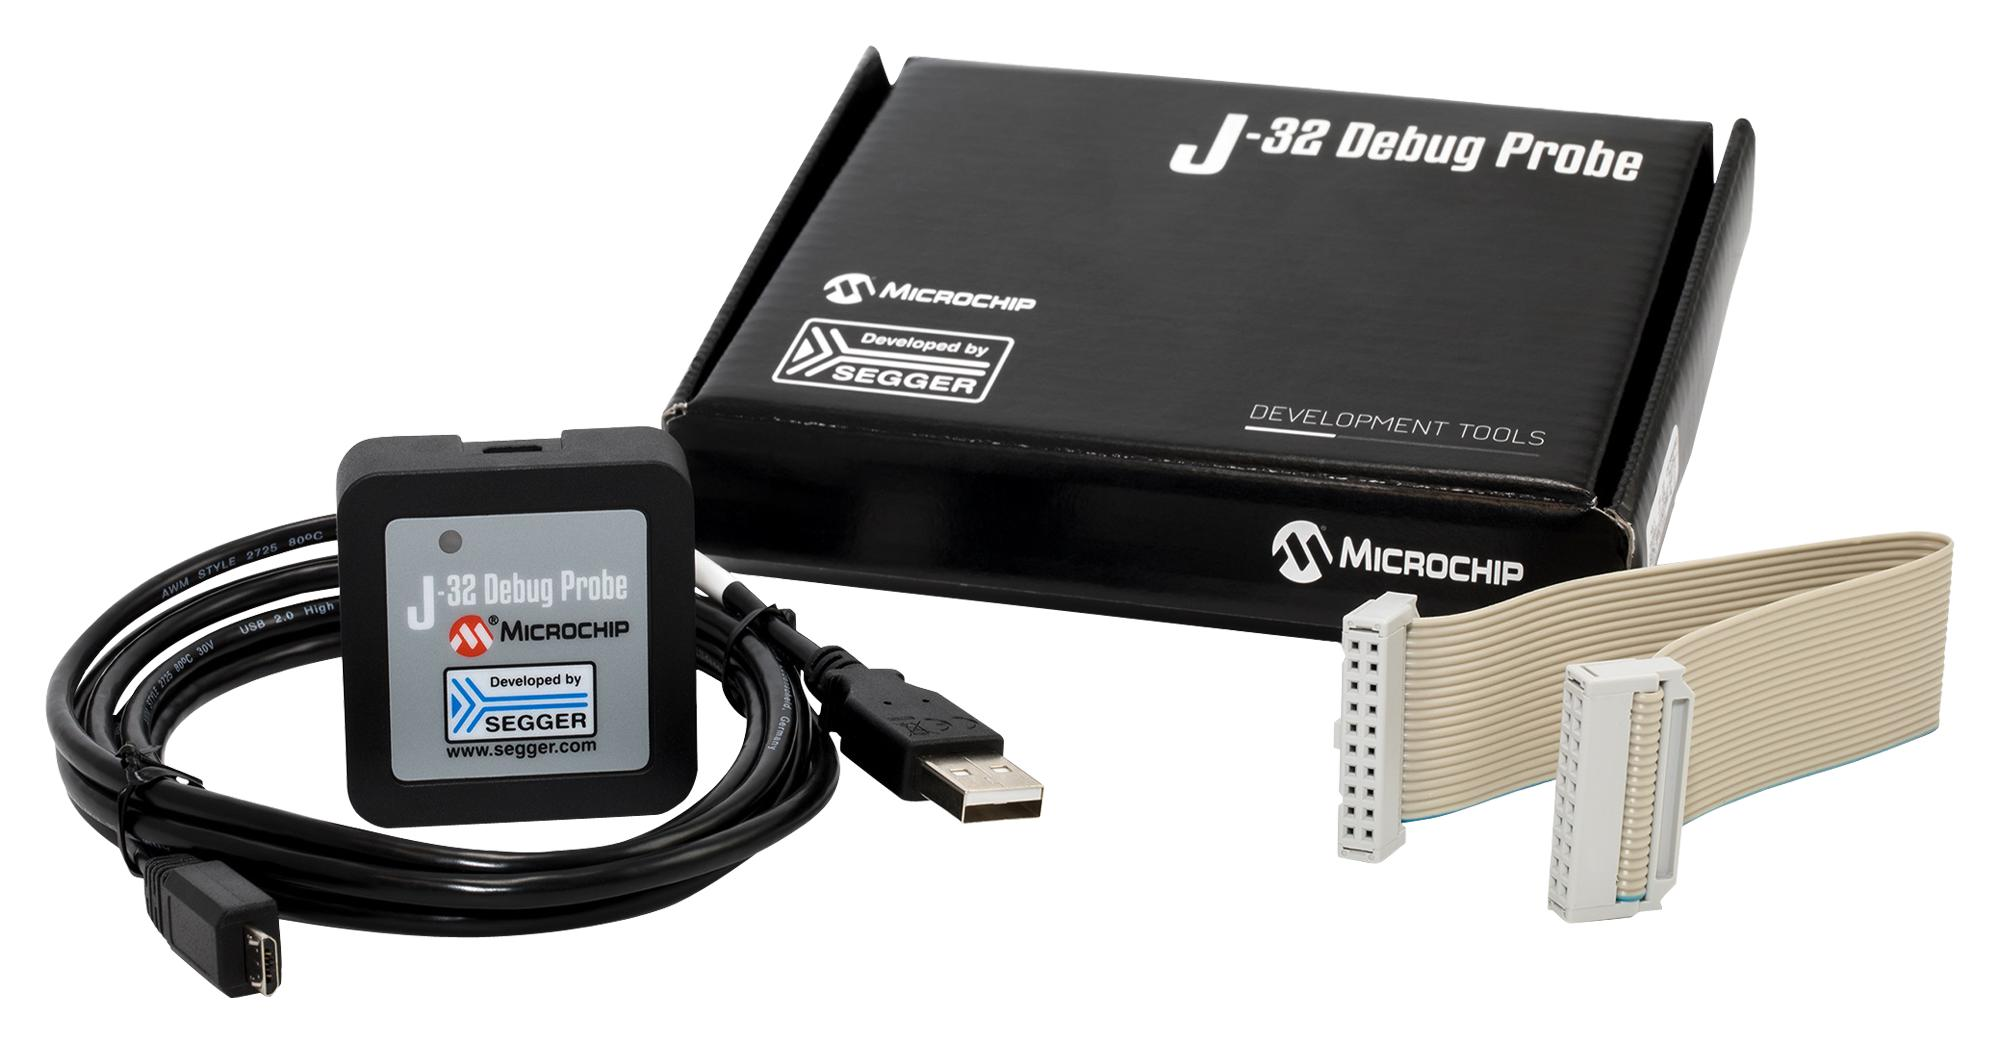
\includegraphics[width=.8\textwidth]{./Figures/segger.jpg}
    \caption{Sonda de depuración \emph{Segger J-32}\protect\footnotemark.}
	\label{fig:sonda}
\end{figure}
\footnotetext{Imagen tomada de \url{https://www.digikey.com/}}

Un servidor \emph{On-chip debugger} tiene la misión de abstraer la conexión la sonda de depuración.
Además, facilita el manejo del ciclo de vida de la sesión y permite usar \emph{software} como \emph{GNU Project debugger}.
Finalmente, es la base de una pila de tecnologías que permite el uso de herramientas como \emph{Eclipse IDE}.
En la tabla \ref{tab:servidores} se puede observar un resumen de los servidores evaluados en el trabajo.

\begin{table}[h]
	\centering
	\caption[Servidores de depuración]{Comparativa entre servidores de depuración}
	\begin{tabular}{l c c c}    
		\toprule
        \textbf{Servidor} & \textbf{API} & \textbf{Acceso}   & \textbf{Licencia}\\
		\midrule
        OpenOCD           & tcl                         & Registros y SDRAM & MIT\\        	
        PyOCD             & Python 3                    & Registros y SDRAM & Apache-2.0\\
		\bottomrule
		\hline
	\end{tabular}
	\label{tab:servidores}
\end{table}

\section{Periféricos de interés}
\label{sec:perifericos}

El dispositivo bajo prueba ofrece una variedad de periféricos para el desarrollo de aplicaciones.
Sin embargo, el cliente manifestó interés solo en los que se nombran a continuación:
\begin{itemize}
    \item CAN: este periférico permite al microcontrolador ser el dispositivo principal en una \emph{Controller Area Network}. La red es de grado industrial y fue diseñada para gestionar una red de sensores en un ambiente automotriz.
    \item PIO: es el puerto de entradas y salidas digitales de propósito general. En el caso del dispositivo bajo prueba, el periférico permite usar circuitos anti rebote, \emph{pull-up} y \emph{pull-down} internos. 
    \item SPI: el periférico permite realizar una conexión del tipo \emph{Serial Peripheral Interface}. Esta conexión es sincrónica y solo apta para distancias cortas.
    \item UART: es un periférico que permite conectarse a puertos y controlar dispositivos serie.
    \item Watchdog: el periférico sirve para detectar un error de ejecución y reiniciar el microprocesador.
\end{itemize}

En la tabla \ref{tab:perifericosresumen} se resume la funcionalidad de cada uno de ellos.

\begin{table}[h]
	\centering
	\caption[Resumen de periféricos]{Resumen de periféricos}
	\begin{tabular}{l c c}    
		\toprule
        \textbf{Periférico} & \textbf{Funcionalidad}\\
		\midrule
		CAN                 & Bus de comunicación de grado industrial\\        	
		PIO                 & Entradas y salidas digitales\\
		SPI                 & Interfaz de comunicación sincrónica\\
		UART                & Puerto para dispositivos serie\\
		Watchdog            & Detección de errores y reinicio del integrado\\
		\bottomrule
		\hline
	\end{tabular}
	\label{tab:perifericosresumen}
\end{table}

\section{Requerimientos del cliente}
\label{sec:emphuerimientos}

Se realizaron una serie de reuniones con el cliente y se pudo definir los requerimientos del trabajo.
A continuación se enumeran los principales:

\begin{enumerate}
	\item Referentes al inyector por consola de comandos:
		\begin{enumerate}
			\item Generará de una interfaz de usuario.
			\item Permitirá configurar el ensayo a realizar.
			\item Observará la salida del dispositivo bajo prueba.
            \item Inyectará \emph{soft-errors} en el dispositivo bajo prueba.
			\item Persistirá las operaciones, entradas y salidas.
			\item Generará informes del ensayo realizado.
		\end{enumerate}
	\item Referentes al proceso del dispositivo bajo prueba:
		\begin{enumerate}
			\item Verificará el estado de los periféricos del dispositivo bajo prueba.
			\item Detectará si el dispositivo bajo prueba perdió su secuencia.
			\item Generará reportes de estado de periféricos y secuencia.
			\item Permitirá que inyector por consola de comandos configure el alcance de la secuencia.
			\item Permitirá que inyector por consola de comandos maneje el flujo de su secuencia.
		\end{enumerate}
\end{enumerate}

El cliente definió algunas restricciones para el desarrollo del sistema.
Estas se enumeran a continuación:

\begin{itemize}
	\item Utilización de un repositorio con control de versiones \emph{Gitlab}.
	\item Documentación del código con \emph{Doxygen}.
	\item Utilización exclusiva del lenguaje de programación \emph{Python 3}.
\end{itemize}

